\begin{figure*}[t]
\centering
\begin{subfigure}[t]{0.24\textwidth}
    \centering
    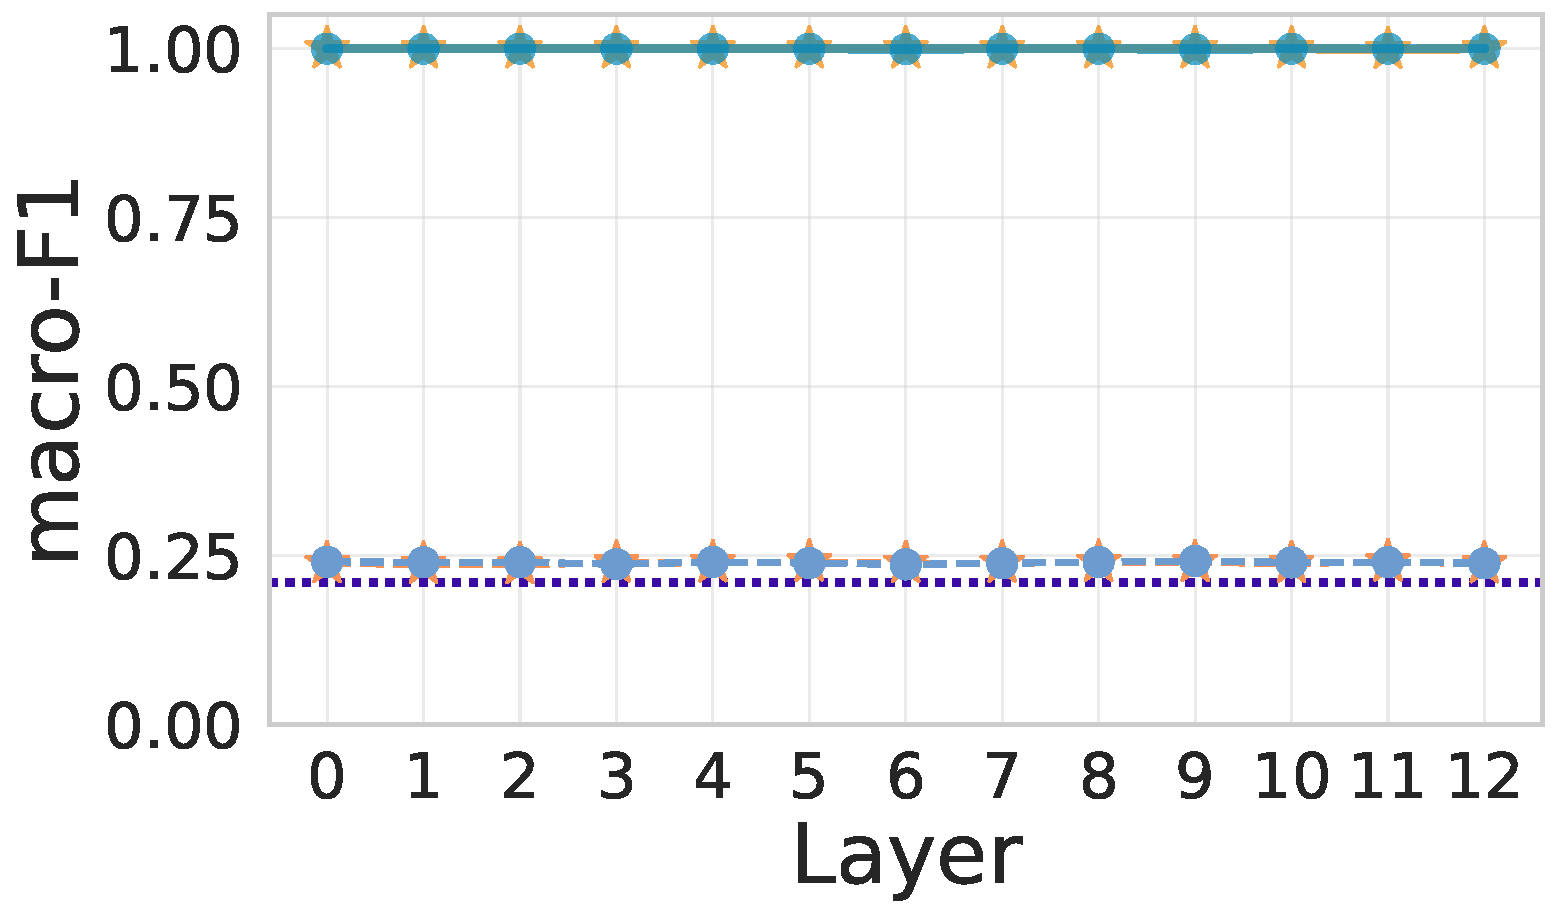
\includegraphics[width=\linewidth]{results_combined_f1/atom_type.pdf}
    \caption{atom type}
\end{subfigure}\hfill
\begin{subfigure}[t]{0.24\textwidth}
    \centering
    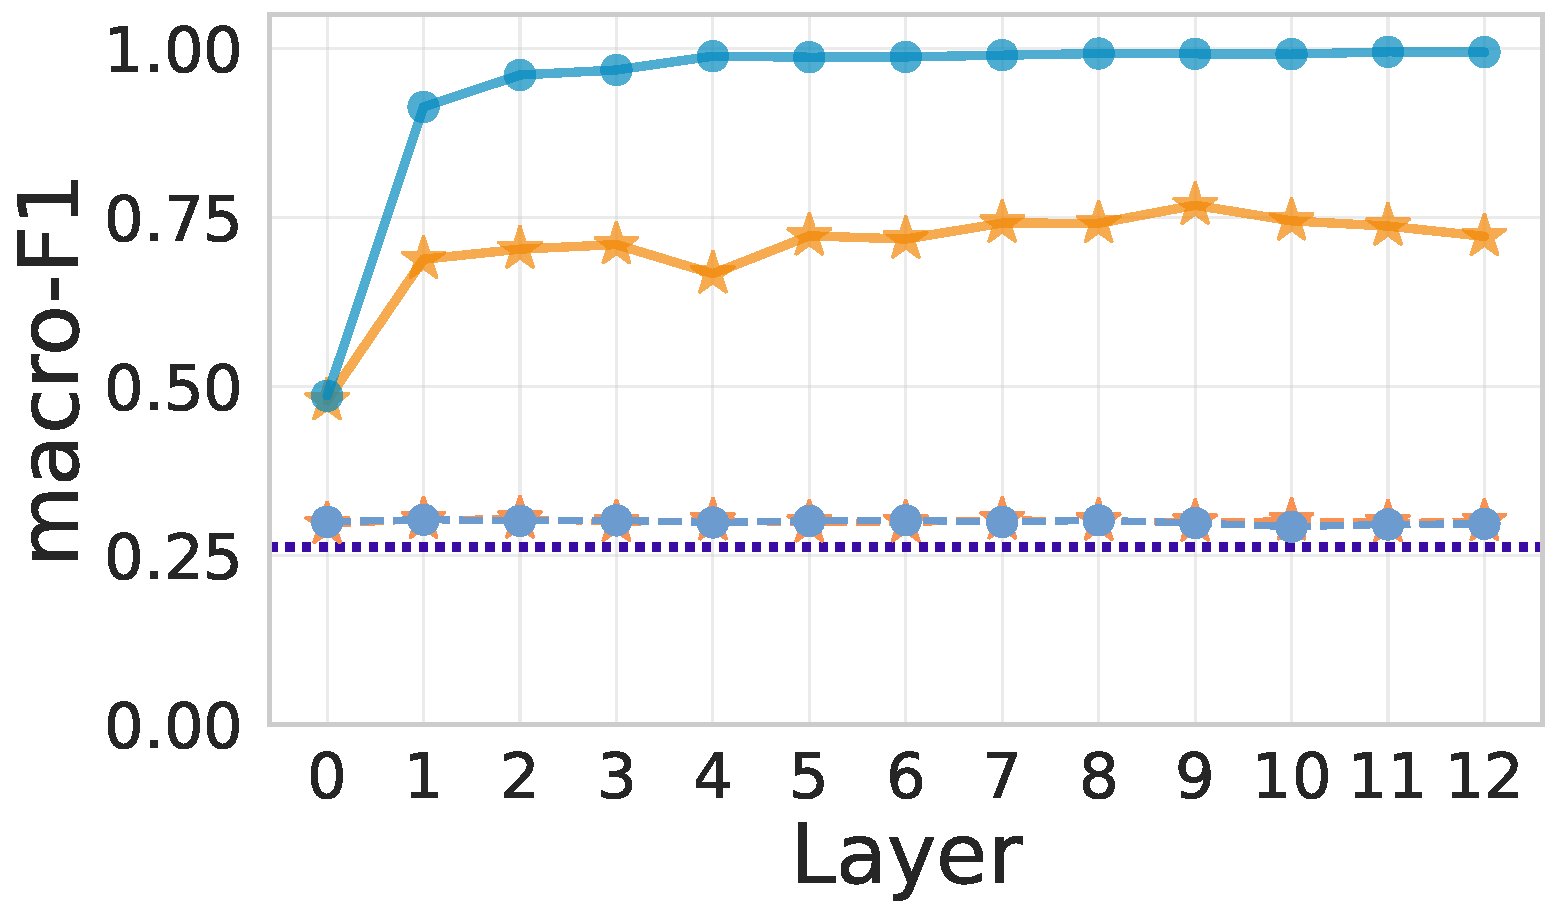
\includegraphics[width=\linewidth]{results_combined_f1/hybridization.pdf}
    \caption{hybridization}
\end{subfigure}\hfill
\begin{subfigure}[t]{0.24\textwidth}
    \centering
    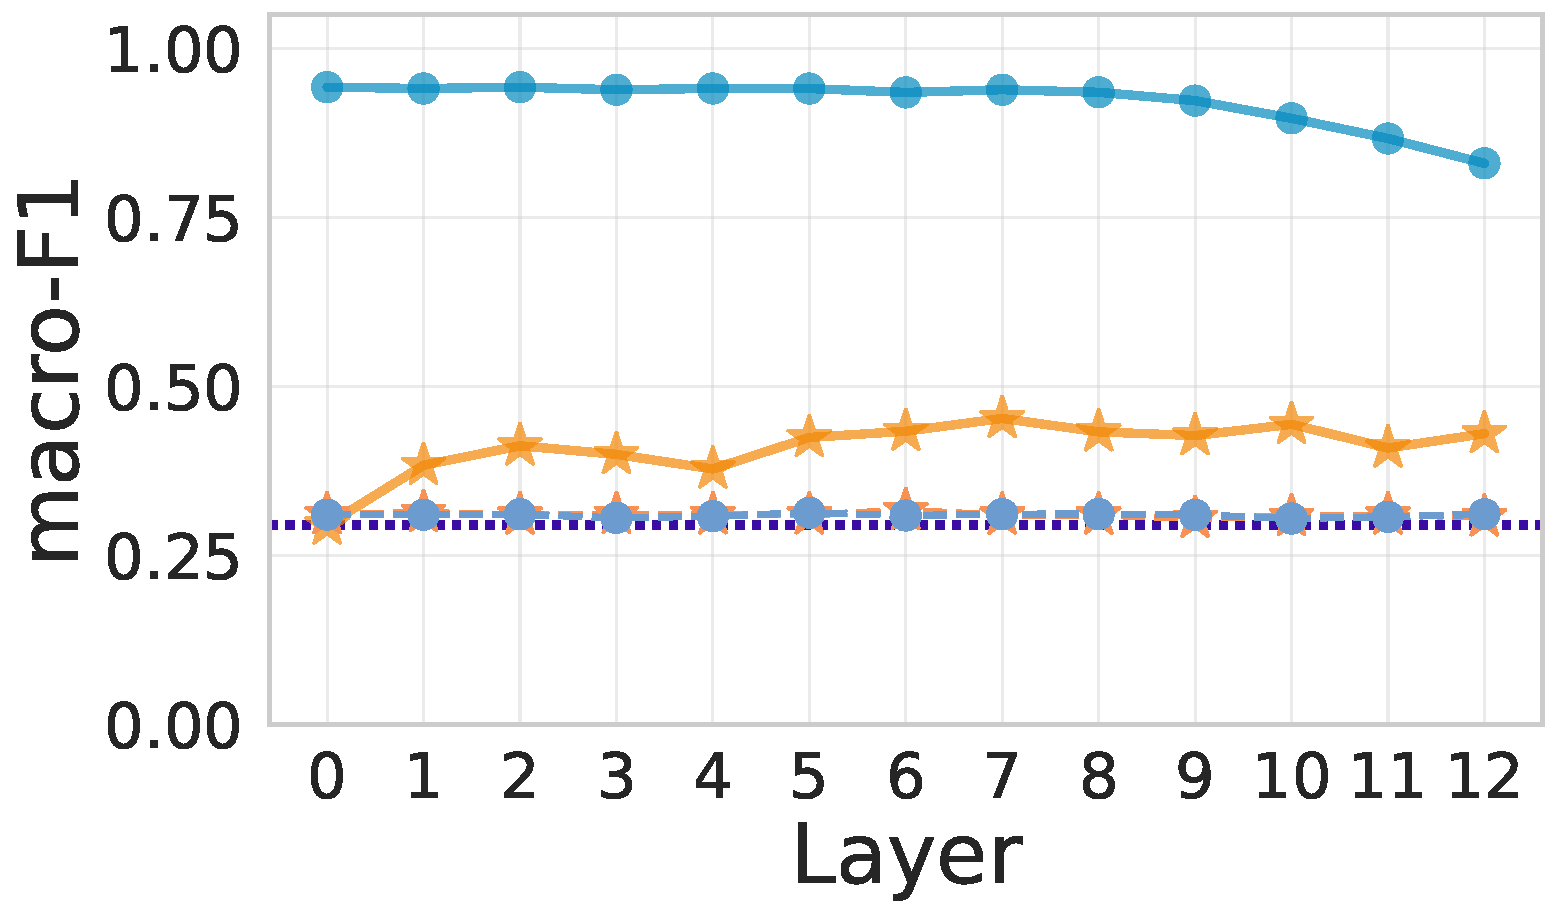
\includegraphics[width=\linewidth]{results_combined_f1/chiral_tag.pdf}
    \caption{chiral tag}
\end{subfigure}\hfill
\begin{subfigure}[t]{0.24\textwidth}
    \centering
    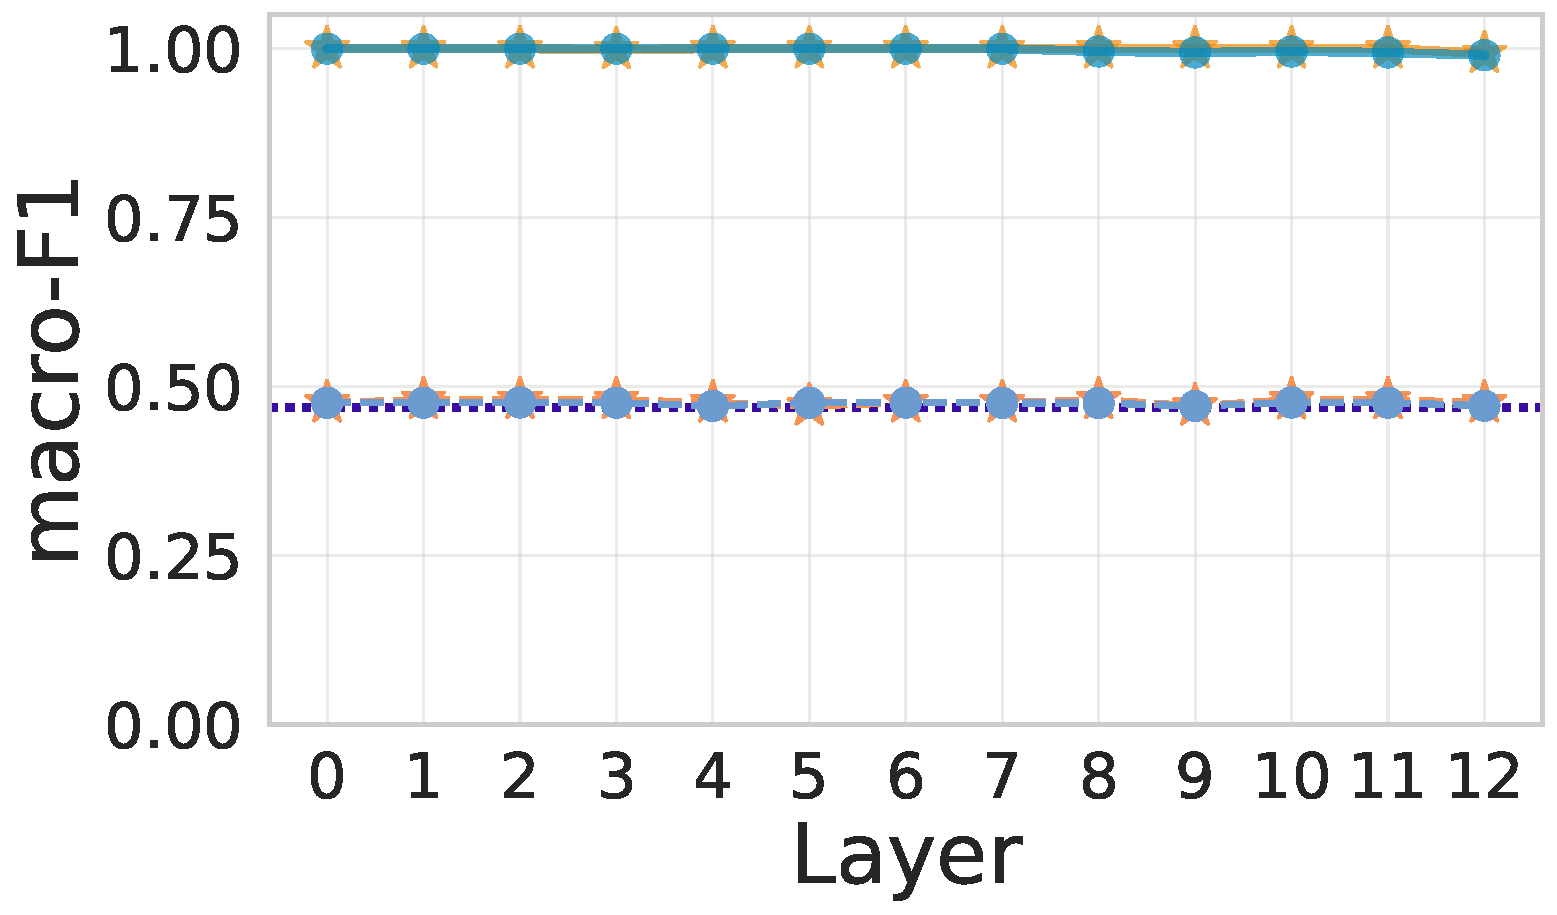
\includegraphics[width=\linewidth]{results_combined_f1/is_aromatic.pdf}
    \caption{is aromatic}
\end{subfigure}

\vspace{0.6em}

\begin{subfigure}[t]{0.24\textwidth}
    \centering
    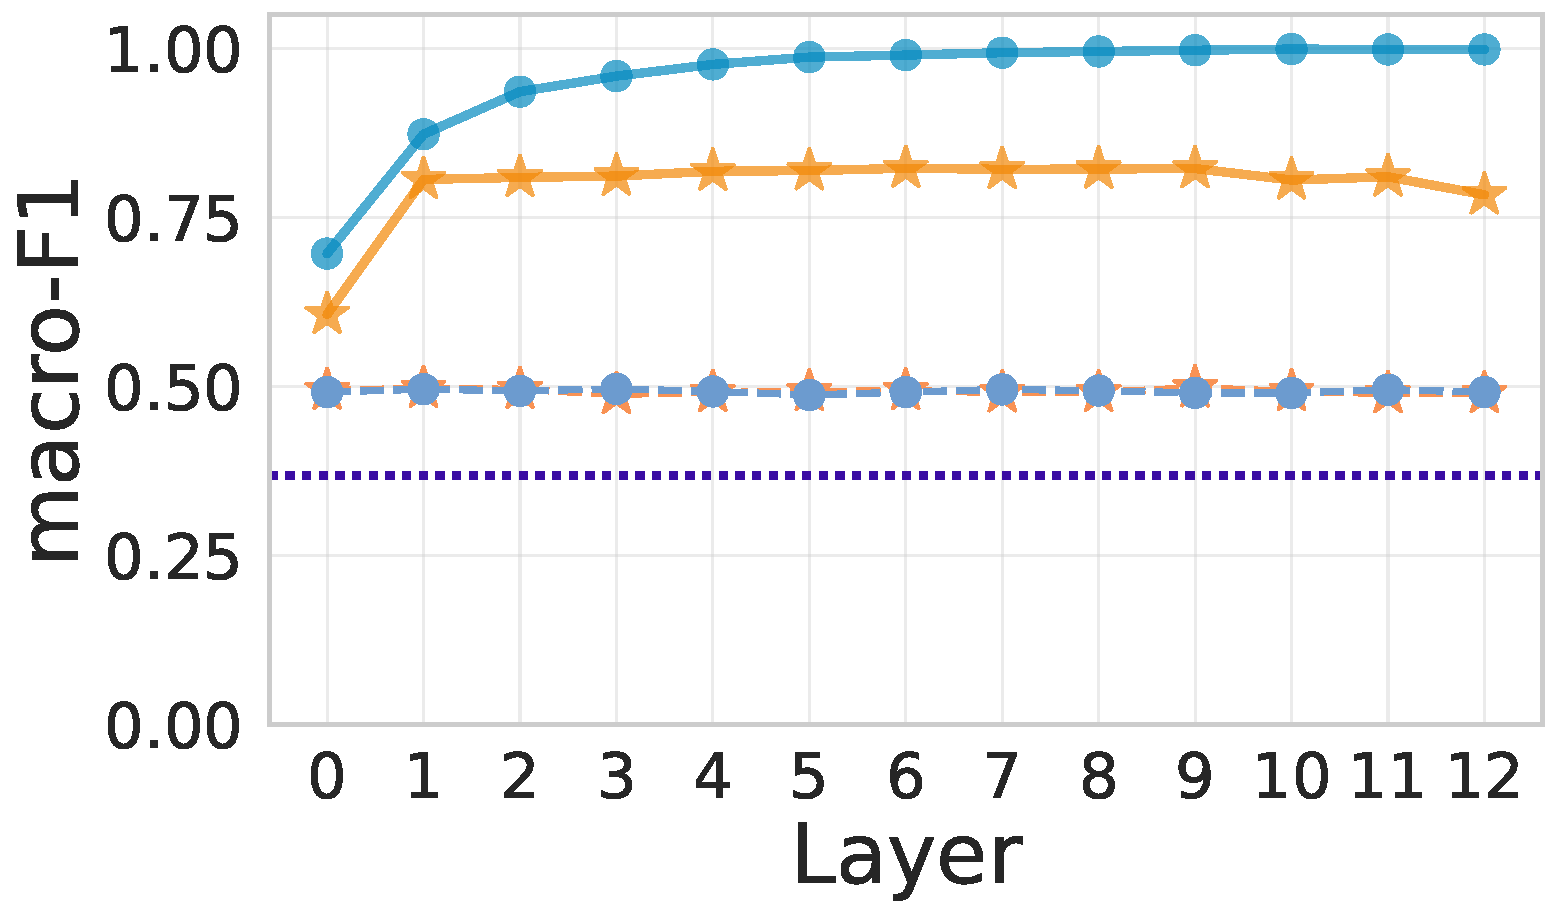
\includegraphics[width=\linewidth]{results_combined_f1/is_in_ring.pdf}
    \caption{is in ring}
\end{subfigure}\hfill
\begin{subfigure}[t]{0.24\textwidth}
    \centering
    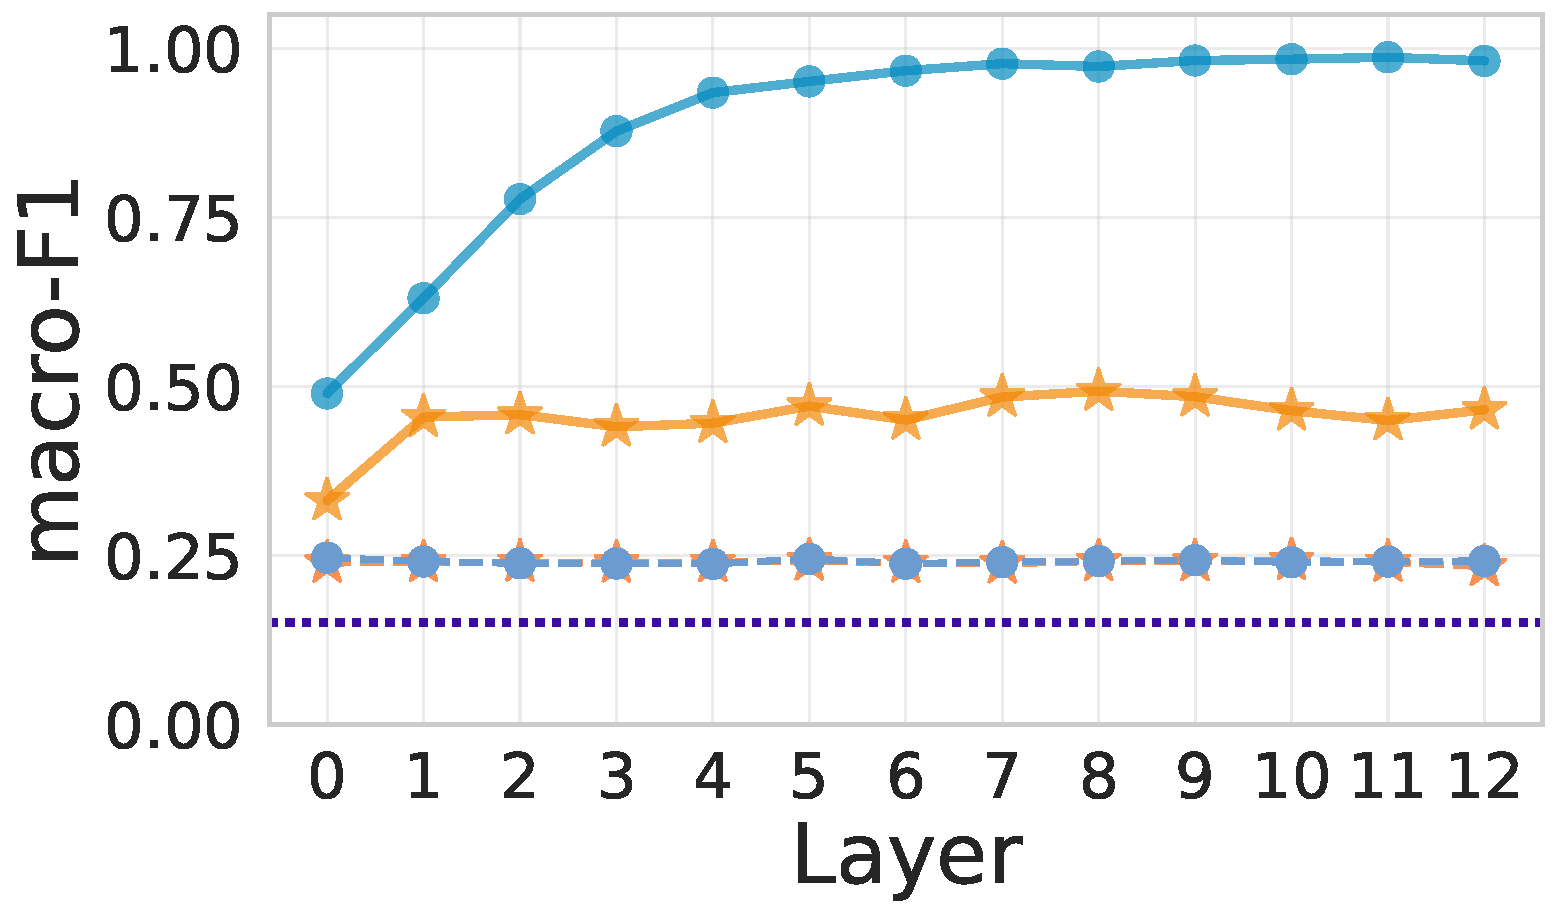
\includegraphics[width=\linewidth]{results_combined_f1/degree.pdf}
    \caption{degree}
\end{subfigure}\hfill
\begin{subfigure}[t]{0.24\textwidth}
    \centering
    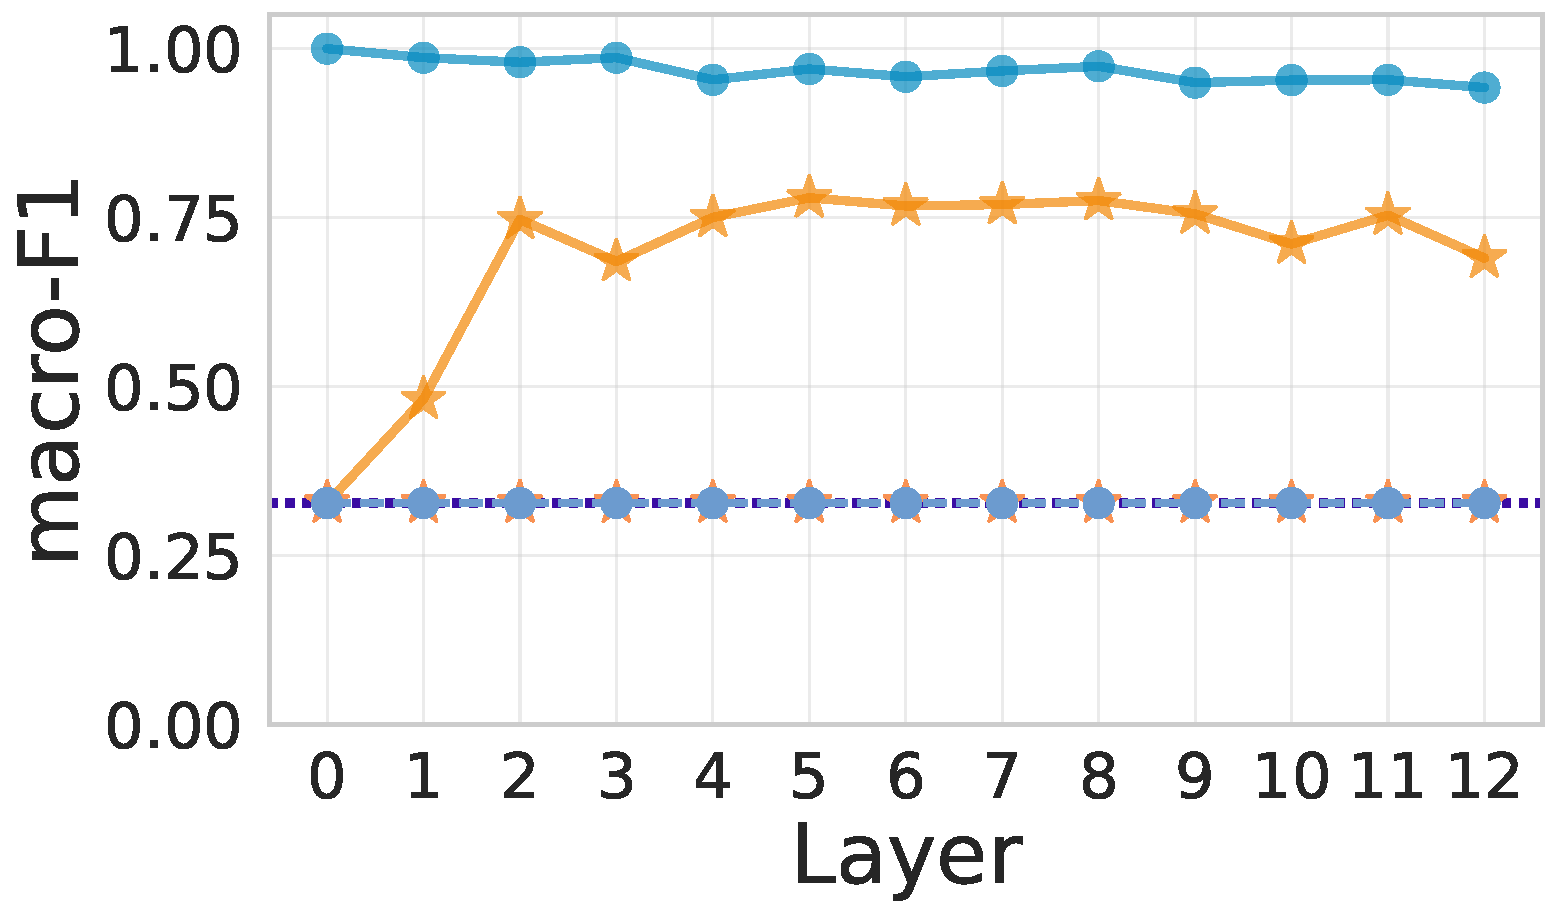
\includegraphics[width=\linewidth]{results_combined_f1/formal_charge.pdf}
    \caption{formal charge}
\end{subfigure}\hfill
\begin{subfigure}[t]{0.24\textwidth}
    \centering
    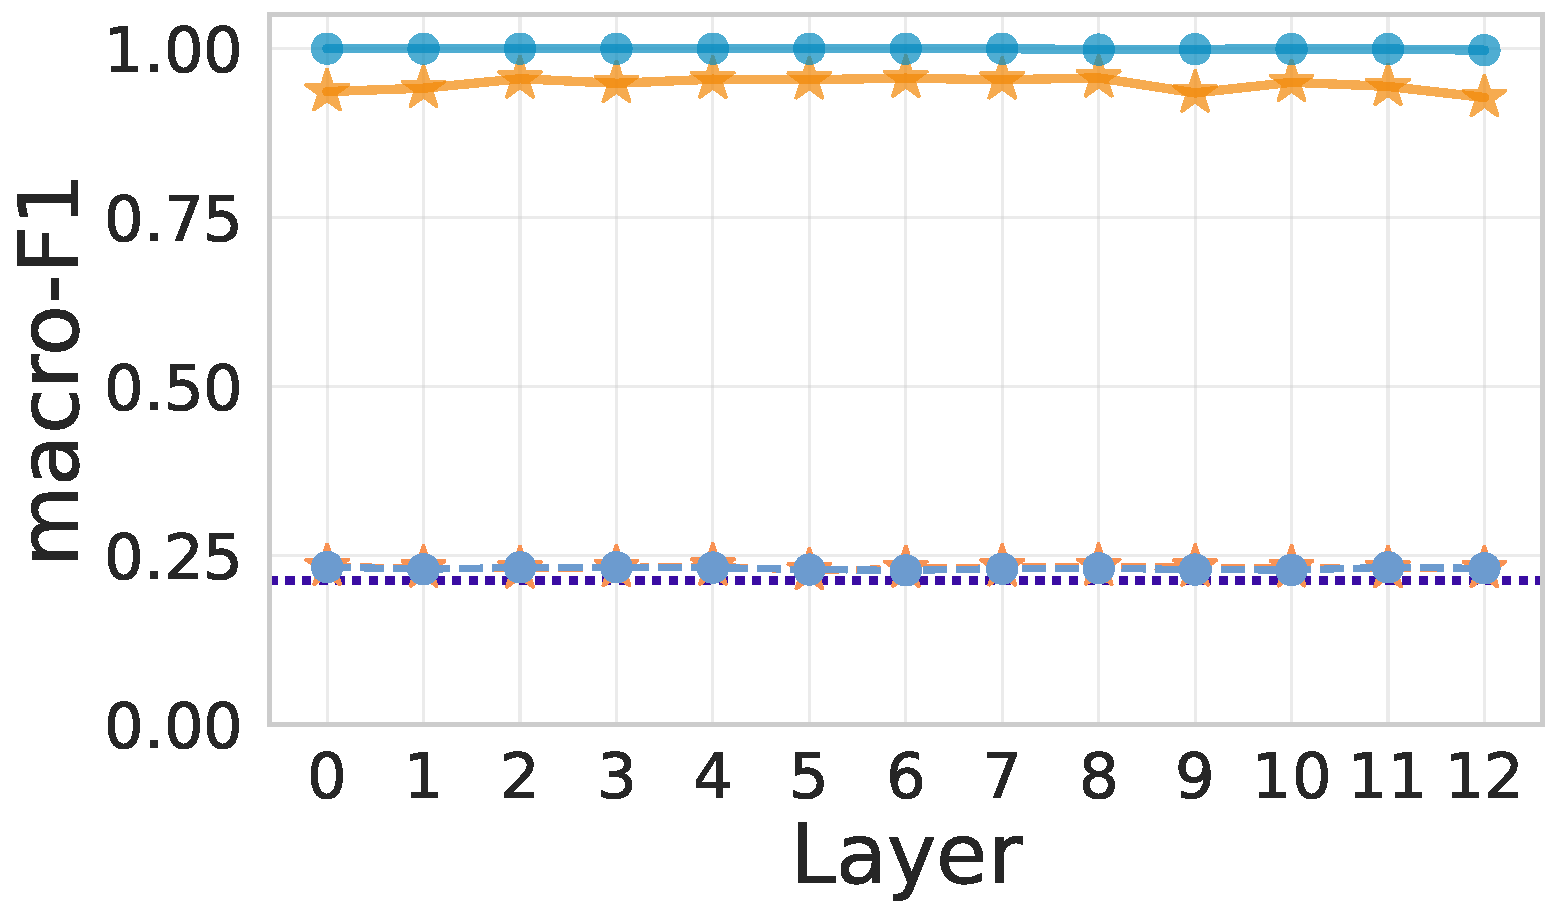
\includegraphics[width=\linewidth]{results_combined_f1/total_valence.pdf}
    \caption{total valence}
\end{subfigure}

\vspace{0.4em}

\centerline{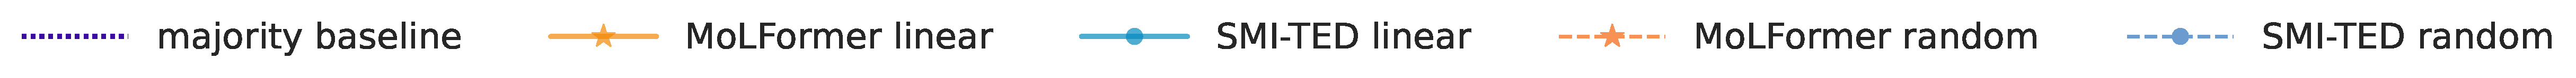
\includegraphics[width=0.95\textwidth]{results_combined_f1/legend.pdf}}

\caption{Per-layer linear-probe macro-F1 on the same eight tasks. Under macro-F1 \smi vs.\ \molm gap on contextual tasks is more pronounced than under accuracy, because macro-F1 penalises probes that effectively predict the majority class.}
\label{fig:f1}
\end{figure*}